\documentclass[useAMS,macros,usenatbib,onecolumn]{mn2e}
\usepackage{multirow}
\usepackage{graphicx}
\usepackage{subfig}
\usepackage{aas_macros}

\title[]{A Spatial FFT and FX Correlator for the BEST-2 Array}
\author[G. Foster, J. Hickish, D. Price and K. Zarb Adami]{G. Foster$^{1}$, J. Hickish$^{1}$, D. Price$^{1}$, K. Zarb Adami$^{1}$\\
$^{1}$Oxford University, Department of Physics}
\begin{document}

\date{\today}

\pagerange{\pageref{firstpage}--\pageref{lastpage}} \pubyear{2011}

\maketitle

\begin{abstract}
A new FX correlator and a spatial FFT imager has been developed using CASPER FPGA hardware for the BEST-2 array at the Radiotelescopi di Medicina in Italy.
Both instruments use the same digitizing/channelizing front end.
The spatial FFT imager takes advantage of BEST-2 as a regularly gridded array to perform a 2D spatial FFT using $O(n \log n)$ operations.
The FX correlator has been used to solve complex gain calibrations which are applied in the spatial FFT during observation.
During the initial deployment of the instruments several bright radio sources were observed over multiple epochs.
%are the sfft images any good?
\end{abstract}

\section{Introduction}

The Basic Element for SKA Training (BEST) 2 array is a subset of the Northern Cross cylindrical array, at the Radiotelescopi di Medicina in Italy.
In this paper we describe a new digital backend designed for this array, implemented on CASPER \citep{casper} designed FPGA-based hardware, and comprising fast correlation, direct imaging, beamforming and transient processing capabilities.

%This digital backend consists of a 32 element digitizer, FX correlator, spatial FFT imager and beamformer implemented on ROACH FPGA boards.
%The Basic Element for SKA Training (BEST) test beds, consisting of BEST-1, BEST-2, and BEST-3lo, were developed as prototype systems for SKA hardware development.
%Simplicity of interfacing with different digital backends was a core component of each design.
%Digital firmware development was designed and tested at Oxford and the designs transferred with minimal changes to the available hardware at Medicina.
%A digital backend was installed during the initial setup of BEST-2 using a previous generation of CASPER FPGA hardware \citep{}.
%This new backend implements the same FX correlator functionality but also provides a high speed 10 GbE output interface for millisecond resolution correlations.
%Along with the correlator a spatial fast Fourier Transform (FFT) imager is incorporated which uses the antenna array grid layout to perform a spatial transform to produce a uniform grid of beams covering the array field of view.
%The imager also has a selectable 10 GbE beam output with can be used with a pulsar processor.
These instruments have been installed as prototypes for larger scale instruments currently in development.
The correlator is being used to study the handling of large output data rates and the development of real time millisecond imaging using many antenna elements.
The direct imaging system is being used to study the feasibility of such systems in arrays with regular geometric structure, as well as providing a platform for pulsar surveys and space-debris tracking capabilities with BEST-2.
%Design and deployment of a prototype design is key to understanding the possible future uses for such an instrument.
Since deployment, a number of sources with the correlator and imager have been successfully observed.
Data has been reduced and calibrated using a combination of custom software and standard radio synthesis imaging packages.

In the first section of this paper we give an overview of the BEST-2 Array, followed by a description of the channelization, correlation and image-domain processing systems in Sections \ref{channelization}, \ref{correlator} and \ref{s-engine}, respectively. Results from preliminary observations of bright radio sources from these systems are presented in Section \ref{results}, with a discussion of these in Section \ref{discussion}.

\subsection{BEST-2 Array}
\label{best-2 array}

The BEST-2 testbed at the Medicina Radio Observatory consists of 8 East-West oriented cylindrical concentrators, each with 64 dipole receivers critically sampling for focal line at 408MHz.
These 64 dipoles are summed in groups of 16, resulting in 4 channels per cylinder, and a total of 32 effective receiving elements laid out on a \emph{4-by-8} grid, fig. \ref{fig:ant_layout}.

BEST-2 was developed as a reliable, low cost frontend to be used in SKA development, with simplicity of interfacing with different digital backends a core design requirement \citep{best2}.
Extensive documentation of the development of the BEST-2 analogue chain can be found in a number of papers \citep{best2-lna} \citep{best2-rec}. The top level specifications of the array are shown in table \ref{tbl:best2}.

%The array has an effective collecting area of approximately 1000 $m^2$ and covers a 16 MHz band centered %at 408 MHz.
%The longest North-South baseline is 70 m and East-West 17 m for a synthesized beam of $0.9$ square %degrees at 408 MHz.
%Further specifications of the array characteristics have been listed in table \ref{tbl:best2}.

In 2008 the initial digital correlator backend of the array was based on iBOB and BEE2 FPGA boards from the Collaboration for Astronomy Signal Processing and Electronics Research (CASPER)\citep{best2-casper}.
An upgraded digital backend has been developed using the ROACH board, also developed by CASPER, which includes an FX correlator, spatial FFT imager and beamformer.

\begin{table}
\begin{center}
\begin{tabular}{| l | l | l |}
\hline
\multicolumn{3}{|c|}{BEST-2 Array Specifications}\\
\hline
Cylinder \& Element Properties & &\\
\hline
Number of RX per Cylinder 	&          4 &            	\\
Cylinder Diameter 		&        7.5 &          m 	\\
Cylinder Length 		&       23.5 &          m 	\\
Element Diameter 		&        7.5 &          m 	\\
Element Length 			&       5.88 &          m 	\\
Element Collecting Area 	&       44.1 &        $m^2$ 	\\
Aperture Efficiency 		&       0.71 &            	\\
Element Effective Area 		&       31.3 &        $m^2$ 	\\
				&            &            	\\
\hline
BEST-2 Array Properties		&            &            	\\
\hline
Number of Cylinders 		&          8 &            	\\
Total Number of RX 		&         32 &            	\\
Total Collective Area 		&     1411.2 &        $m^2$ 	\\
Total Effective Area 		&    1001.95 &        $m^2$ 	\\
Sensitivity / Ant. gain 	&       0.36 &       K/Jy 	\\
$A_{eff}/T_{sys}$ 		&      11.65 &      $m^2/K$ 	\\
Antenna Temperature 		&         35 &          K 	\\
Receiver Temperature 		&         51 &          K 	\\
System Temperature  		&         86 &          K 	\\
				&            &            	\\
\hline
Longest Baseline 		&            &            	\\
\hline
E-W 				&      17.04 &         m 	\\
N-S 				&      70.00 &         m 	\\
				&            &            	\\
\hline
Bandpass        		&            &       		\\
\hline
Central Frequency 		&        408 &        MHz 	\\
Analog Bandwidth 		&         16 &        MHz 	\\
				&            &            	\\
\hline
Pointing Limits 		&            &            	\\
\hline
Declination 			&    (0,+90) &        deg 	\\
Right Ascension 		&    Local Meridian &  		\\
				&            &            	\\
\hline
Primary Beam 			&            &           	\\
\hline
Primary Beam Size 		&      37.62 & $\textrm{deg}^2$ \\
Declination 			&        5.7 &        deg 	\\
Right Ascension 		&        6.6 &        deg 	\\
				&            &            	\\
\hline
PSF    				&            &       		\\
\hline
PSF FWHM 			&        0.9 & $\textrm{deg}^2$ \\
Declination 			&       0.52 &     deg 		\\
Right ascension 		&       1.73 &     deg 		\\
				&            &            	\\
\hline
\end{tabular}
\caption{The top level specifications of the BEST-2 Array, a subset of the collecting area of the Northern Cross, located in Medicina, Italy.}
\label{tbl:best2}
\end{center}
\end{table}

\begin{figure}
    \centering
    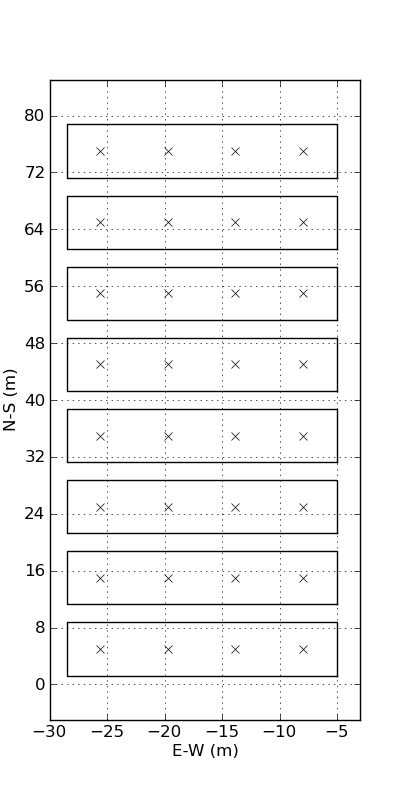
\includegraphics[scale=0.6]{graphics/layout.png}
    \caption{The 32 effective receiving elements of BEST-2, indicated by crosses, lie on a regular 4x8 grid. Each receiver is the analogue sum of 16 dipoles, critically spaced at 408MHz in the East-West direction.}
    \label{fig:ant_layout}
\end{figure}

\section{Instrument Design}
\label{instrument design}

An FX correlator and spatial FFT imager instrument have been built for BEST-2.
Both instruments use the same digitization and channelization frontend.
This allow a streamlined process of calibrating the spatial FFT imager, reduces the amount of hardware and allows for simultaneous observation with both instruments.
The instrument has been implemented on ROACH boards which are a generic field programmable gate array (FPGA) board designed by CASPER for radio astronomy applications.
A ROACH consist of a XILINX Virtex 5 SX95T FPGA with interfaces to DRAM and QDR memory, high speed CX-4 connectors and a generic Z-DOK interface for connecting ADCs and various daughter boards, fig \ref{fig:roach}.
Additionally, the board has a PowerPC running BORPH, a variant of Debian Linux, which allows access to software registers and shared memory on the FPGA.
Firmware is designed using MATLAB Simulink which is extended with XILINX DSP blocks and CASPER's open source DSP blocks\citep{}.
Design specific DSP blocks and hardware interfaces have also created, design models and control software are available from our project repository\footnote{https://github.com/griffinfoster/medicina}.
Instrument design specifications are presented in table \ref{tbl:digital_specs}, further design detail is described in the following sections.

\begin{figure}
    \centering
    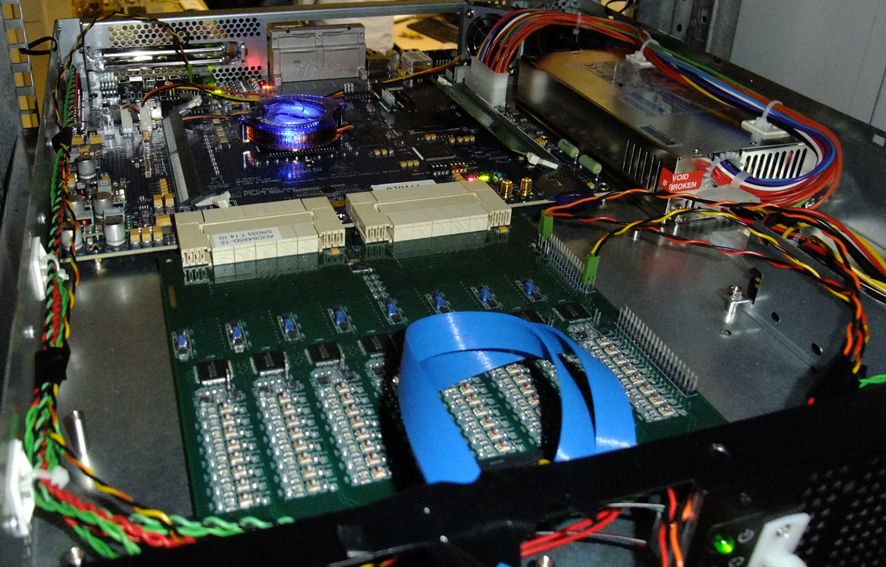
\includegraphics[scale=0.4]{graphics/roach_feng.png}
    \caption{The 'f-engine' ROACH board, a Virtex 5 SX95T FPGA board, with the 64 input ADC connected via two Z-DOK connectors.}
    \label{fig:roach}
\end{figure}

\begin{table}
\begin{center}
\begin{tabular}{| l | l | l |}
\hline
\multicolumn{3}{|c|}{Digital Backend Specifications}\\
\hline
Digitizer/Channelizer (F-Engine) & &\\
\hline
ADC Sampling Rate	& 40 			& MHz\\
ADC Sampling Precision	& 12 			& bit \\
Antenna-polarizations 	& 32 			& single pol \\
PFB 			& 4 tap FIR + 2048 point FFT	& Radix-2 Biplex Real FFT\\
%FFT 			& 2048 point 		& Radix-2 Biplex Real\\
Quantization 		& 4 			& bit\\
& & \\
\hline
FX Correlator (X-Engine) & &\\
\hline
Auto Correlations 	& 32 			& \\
Cross Correlations 	& 496 			& \\
Minimum Integration Length & 6.55 		& ms\\
Output 			& 10 GbE 		& SPEAD protocol\\
& & \\
\hline
Spatial FFT Imager (S-Engine) & &\\
\hline
2D FFT 			& 8 x 16 		& \\
Beams 			& 128 			& \\
Minimum Integration Length & 1 			& s\\
Output 			& 1 GbE 		& SPEAD protocol\\
Beamformer Output 	& 10 GbE 		& Up to 8 Beams\\
& & \\
\hline
\end{tabular}
\caption{A three ROACH design where the correlator and spatial FFT imager use the digitizer/channelizer interface.}
\label{tbl:digital_specs}
\end{center}
\end{table}

\subsection{Digitization and Channelization}
\label{channelization}

Signal digitization is performed using the Texas Instruments ADS5272 8 channel, 12 bit ADC.
The ADC board, developed by Rick Raffanti \citep{}, uses eight of these ADCs to channelize 64 streams at up to 65 Msps.
In our design only 32 signal streams are digitized at 40 Msps which more then covers the 16 MHz analog band.
The ADC is clocked with a 160 MHz clock which is locked to a local maser source.
During the analog stage the RF, centered at 408 MHz, has been mixed down to baseband.
Prior to digitization the last amplifier stage of the analog chain has per signal adjustable gain useful for setting good levels for ADC quantization.
This ADC is connected via a dual Z-DOK interface to an 'F-Engine' ROACH which performs the channelization.
The ROACH board is clocked at four times the sample rate such that four signals are time division multiplexed onto a single stream.
Channelization is performed with a four tap Hann filter, 2048 point polyphase filterbank (PFB) to produce 1024 samples per real antenna stream.
The CASPER PFB has been modified to account for the signal multiplexing.
Each channel has a width of 19.5 kHz and the output of the FFT stage is a 36 bit complex number.
The narrow channel widths and PFB windowing allows for good frequency separation in the high RFI environment at the observatory.
After channelization the samples are quantized down to a 8 bit complex number.
An adjustable, per channel complex gain equalizer is used for amplitude and phase corrections before quantization.
Complex gain calibration is essential to proper spatial FFT imaging which must be applied before the spatial FFT.
The FX correlator is used to generate calibration coefficients which are applied back into the equalizers.
A selectable mux is available to skip the phase coefficients on the FX correlator data stream.
Post equalization the data stream is split into two for specific reordering for the correlator and imager.
The correlator data stream is reordered to 128 time samples for a single antenna for a single frequency channel.
Followed by the next antenna and cycles back onto the next frequency channel.
The imager takes in one time sample of each antenna for a given frequency channel and cycles through 128 time samples before stepping to the next frequency channel.
After data reordering each stream is sent over high speed XAUI at a rate of 5.12 Gbps to the correlator and imaging boards.

\begin{table}
\begin{center}
\begin{tabular}{| l | l | l |}
\hline
\multicolumn{3}{|c|}{F-Engine ROACH Resource Utilization (Virtex 5 SX95T)}\\
\hline
ADC Clock 		& 40 MHz \\
System Clock 		& 160 MHz 	& Demux:4 \\
Slice Registers 	& 30217 / 58880 & $51\%$\\
Look Up Tables 		& 24319 / 58880 & $41\%$\\
BRAM (36kb) 		& 205 / 244 	& $84\%$\\
DSP48e (Multipliers) 	& 185 / 640 	& $28\%$\\
CX-4 Interface 		& 2 / 4 	& 5.12 Gbps XAUI\\
QDR Memory 		& 2 / 2 	& Cornerturn\\
\hline
\end{tabular}
\caption{DSP implementation of the 'f-engine'}
\label{tbl:feng_resource}
\end{center}
\end{table}

\begin{figure}
    \centering
    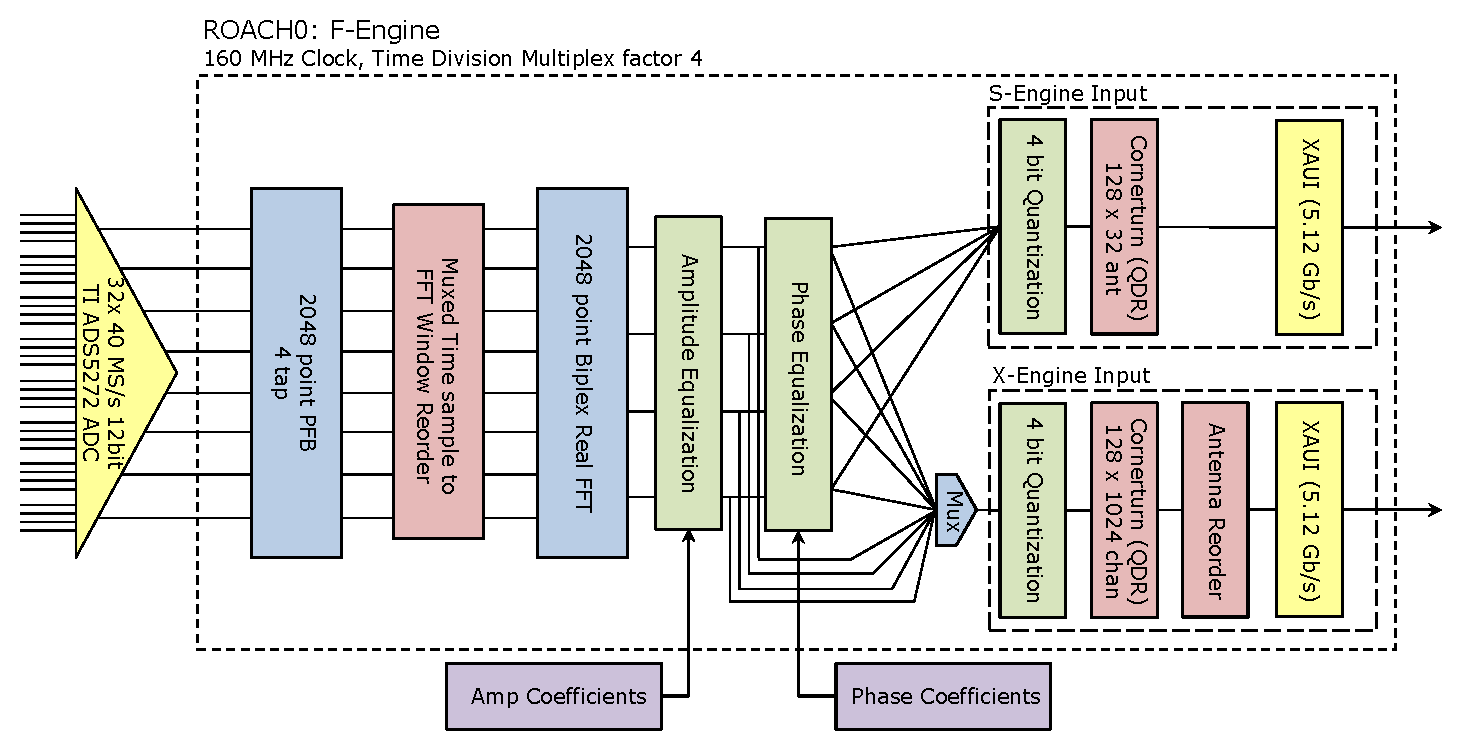
\includegraphics[scale=0.6]{graphics/crop_fengine_block.pdf}
    \caption{During observations amplitude and phase coefficients are applied to scale the power for the 4 bit correlation and apply phase corrections for the spatial FFT.}
    \label{fig:feng_block}
\end{figure}

\subsection{FX Correlator}
\label{correlator}

An FX correlator design is a standard design for large bandwidth and many antenna arrays.
The F component represents the frequency channelization, and the X is a complex multiply and accumulate (CMAC).
An overview of the architecture is presented in \citep{}.
Architecture efficiency goes as $O( M \textrm{log} M) + O( N^2)$ where $M$ is the number of FFT frequency channels and $N$ is the number of antenna-polarizations.
The core component to the X stage of the FX correlator is the complex multiplication of all pairs of independent signals for each frequency channel.
A pipelined x-engine, based on the general CASPER block originally designed by Lynn Urry\citep{}, is used for multiplier efficiency.
The pipeline design is constructed out of $M/2$ 'taps' where the $i^{th}$ tap computes the correlation between antennas $A_j$ and $A_{j+i}$ for every antenna $A_j$ of $M$ total antennas.
To maximize the multiplier usage a loopback is added to use every $i^{th}$ tap to compute the correlation of antennas $A_j$ and $A_{M/2+j+i}$, fig. \ref{fig:xeng_pipe}.
Each tap accumulates for $N$ time samples to reduce the output data rate.

\begin{figure}
    \centering
    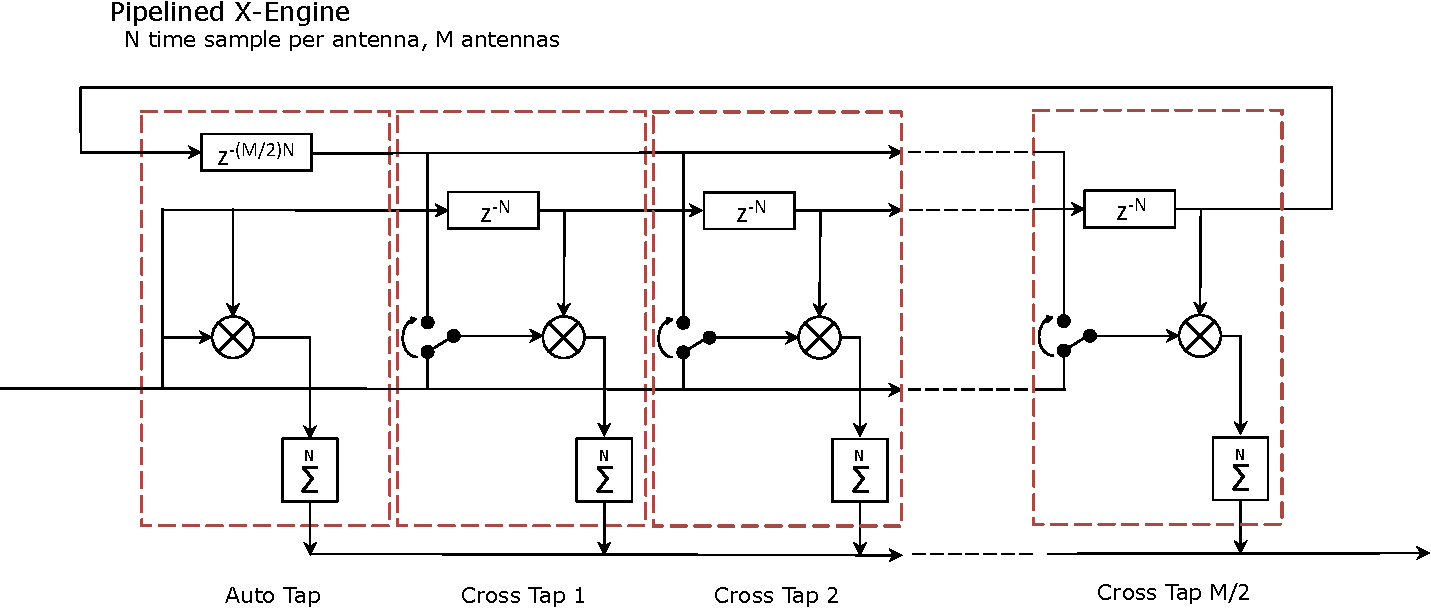
\includegraphics[scale=0.6]{graphics/crop_pipelined_xeng.pdf}
    \caption{The input is ordered as $N$ time samples per antenna per frequency channel. An accumulation stage after the complex multiply reduces the data rate of each tap. Outputs are multiplexed onto the same output using a valid signal.}
    \label{fig:xeng_pipe}
\end{figure}

An asynchronous architecture is used between the f-enigne and x-engine boards.
The x-engine board has been clocked to 200 MHz, well above the 160 MHz f-engine board, this assures the x-engine board will never have input buffer overflows during the windowing stage.
The XAUI interboard connection is a streaming interface which guarantees the same output order as input order but with variable latency.
In rare cases the XAUI interface can drop 64 bit words during the streaming, this requires an initial stage to track the number of words received between headers.
In case of missing words the entire payload is dropped and counters reset for the next header.
A correlation is only performed on a per channel basis.
The channelized band can be split up into portions and processed in parallel across multiple x-engines.
This allows a larger bandwidth to be processed at the cost of increased logic and multiplier resource utilization.
For this design two x-engines are used which each processes half of the band.
The x-engine design requires a continuous stream of data for 128 samples of all antennas for a single frequency channel.
Prior to the x-engine samples are buffered up into windows to guarantee valid data during a cycle of the x-engine.
For reasons related to the design the 32 single polarization signals are treated as 16 dual polarization signals.
This causes a small number of redundant baseline correlations and a conjugation effect which is corrected in post processing.
During the x-engine stage an initial accumulation of 128 sample is performed after the complex multiply to reduce the output rate to roughly the input rate.
This limits the minimum integration time to 6.55 ms.
A vector accumulator using the on board QDR memory is used for longer integration lengths.
This second accumulator is software controlled with integration lengths ranging from milliseconds to minutes.
A completed integration is sent to a receive computer over a 10 GbE connection.
Integrations are split up based on the SPEAD protocol\citep{} and transmitted as UDP packets.

\begin{table}
\begin{center}
\begin{tabular}{| l | l | l |}
\hline
\multicolumn{3}{|c|}{X-Engine ROACH Resource Utilization (Virtex 5 SX95T)}\\
\hline
System Clock & 200 MHz \\
Slice Registers & 28494 / 58880 & $48\%$\\
Look Up Tables & 25349 / 58880 & $43\%$\\
BRAM (36kb) & 88 / 244 & $36\%$\\
DSP48e (Multipliers) & 288 / 640 & $45\%$\\
CX-4 Interface & 1 / 4 & 5.12 Gbps XAUI\\
QDR Memory & 2 / 2 & Vector Accumulator\\
\hline
\end{tabular}
\caption{DSP implementation of the 'x-engine'}
\label{tbl:xeng_resource}
\end{center}
\end{table}

\begin{figure}
    \centering
    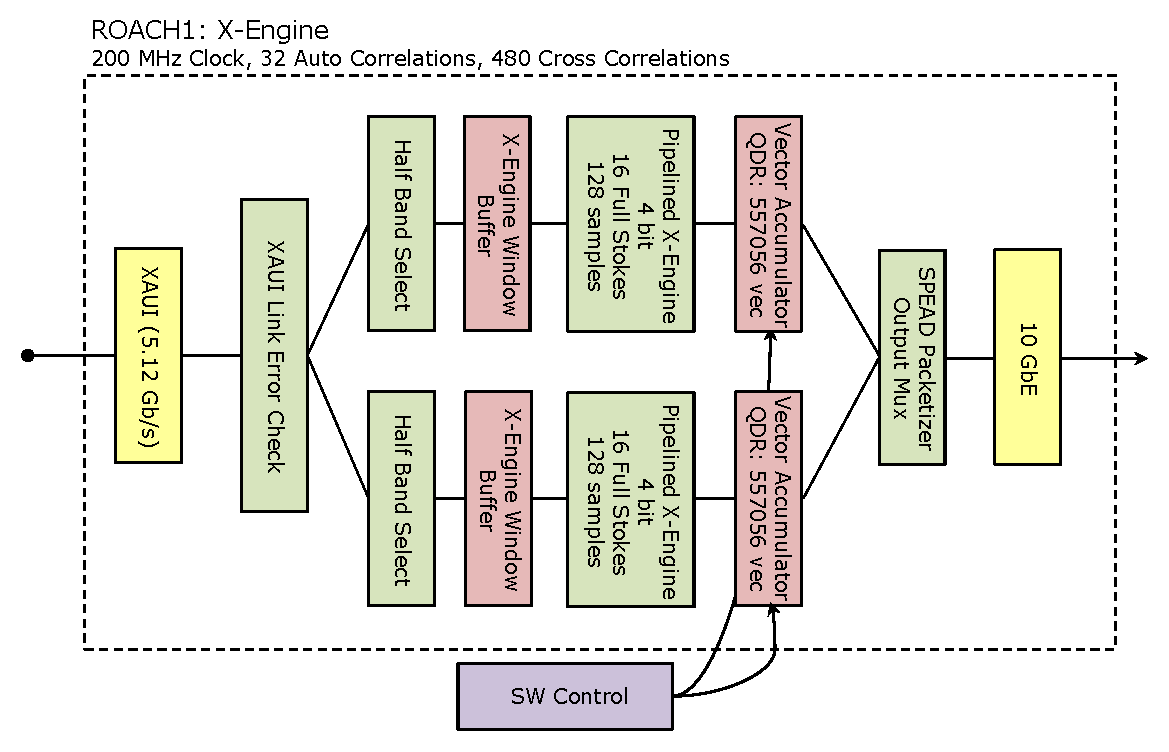
\includegraphics[scale=0.6]{graphics/crop_xengine_block.pdf}
    \caption{Two parallel pipelined x-engines are used, each processes half of the band.}
    \label{fig:xeng_block}
\end{figure}

\subsection{Spatial FFT}
\label{s-engine}
 
When $N$ receiving elements in an antenna array are placed on a regularly spaced grid, a well known method for producing a complete set of orthogonal beams on the sky is the spatial fast Fourier transform \citep{fastbeamforming}.
Such a beamforming implementation will generate $N$ beams on the sky, with a computational cost of $O(N\log{N})$. For large arrays, where many beams are desired, this can be a significant computational saving, with the alternative, so-called \emph{DFT beamforming}, requiring $O(N)$ operations per synthesized beam.
To date, the largest such astronomical implementation of such a spatial fast Fourier transform beamformer is the 64 element dish array constructed in 1994 at Waseda University, Japan \citep{2dfft}.

More recently, spatial FFT based processing has been revisited in the literature with an emphasis on the correlation matrix, rather than the collection of beams, as the mathematical object of interest \citep{fftt} \citep{omniscope}.
In the method outlined by Tegmark \& Zaldarriaga, zero padding is applied to the matrix of antenna signals before the spatial FFT is performed, and as such, the complete set of visibilities for all unique baselines in the array can be obtained, post integration, by inverse Fourier transform.
Conversely, in the image plane, the zero-padding required by the prescribed algorithm results in the generation of $~2^{m}N$ beams on the sky and is dependent on the number of dimensions, $m$, in the antenna array.
Regardless of potential downstream visibility domain processing, this oversampling of the sky by a factor $2^{m}$ has the benefit of increasing the instantaneous uniformity of sky coverage by synthesized beams, which somewhat alleviates the limitations associated with the inability to steer multiple beams independently.

%A spatial FFT imager is a novel instrument which takes advantage of the baseline redundancy in a regularly gridded array to reduce the correlator cost of an FX design $O(n^2)$ to a FFT cost of $O(n \log{n})$.
%Correlation of all antenna pairs in a regularly gridded array makes redundant measurements for many of the baselines.
In the BEST-2 backend described here, the requirements on the spatial FFT processor were multifold. Firstly, the system should be capable of generating images on an $O(\mathrm{second})$ timescale, by the method described by \citep{fftt}. Further, the system should be capable of passing formed beams at full bandwidth, i.e. without any accumulation, to downstream time domain processing systems such as the real-time dedispersion engine \citep{dedispersion}. 


This redundancy for the BEST-2 array is show in figure \ref{fig:redbl}.
Instead of making individual correlations of the same baseline as in an FX correlator the correlation of the average of each baseline can be computed.
This optimization realizes on the assumption that each redundant baseline measurement is indeed identical.
Thus any calibration to the complex gains must be applied before the spatial FFT.

\begin{figure}
    \centering
    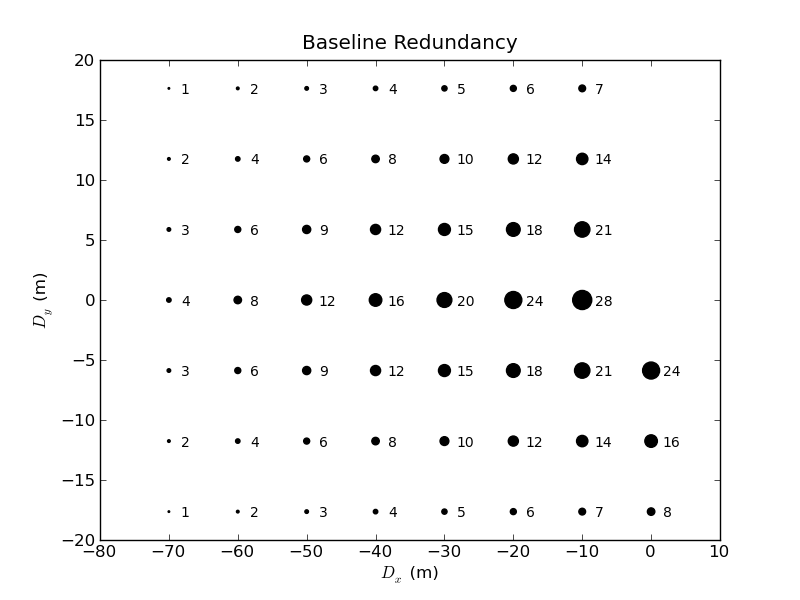
\includegraphics[scale=0.6]{graphics/redbl.png}
    \caption{A 4 by 8 regularly gridded array has 52 unique baselines, 480 cross correlations are performed. The number of redundant baseline measurements is shown as the color and size of each circle.}
    \label{fig:redbl}
\end{figure}

Though the X-Engine and S-Engine use the same F-Engine each requires a unique data windowing order.
For the S-Engine a window is made up of N antennas by M time samples for a given frequency channel.
A similar XAUI interface and windowing scheme is used as in the X-Engine which buffers up windows of valid data to stream into the spatial transform.
The 2D spatial transform is performed using an 8 point FFT followed by a cornerturn and 16 point FFT.
The BEST-2 array is a grid of 4 by 8 antennas, the data is zero padded before input into the 8 by 16 point spatial transform.
A 4 by 8 point spatial transform will only produce gain information for each spatial position, which can be interpreted as an array of beamformers covering the field of view.
This zero padding is necessary to produce both the gain and phase information of each spatial position which is an effective baseline.
Each effective baseline is an average of all possible baselines with the same spatial dimensions.
The four fold increase is the number of outputs from the spatial transform by double padding introduces a number of redundant calculations.
The spatial transform produces 128 outputs, there are only 53 unique baselines in a 4 by 8 grid.
The datarate out of the S-Engine is reduced by a two stage vector accumulator.
A fixed 128 sample vector accumulator reduces the output of the second stage FFT so that the 1024 channels of the 128 computed spatial components can be multiplexed onto one line and accumulated in a software controllable QDR vector accumulator.
Accumulations are sent out over the 1 GbE PowerPC interface using the a SPEAD UDP packet format.
Individual beams can be selected out before accumulation and sent over 10 GbE in a LOFAR beam packet format which will be used for future pulsar processing.

\begin{figure}
    \centering
    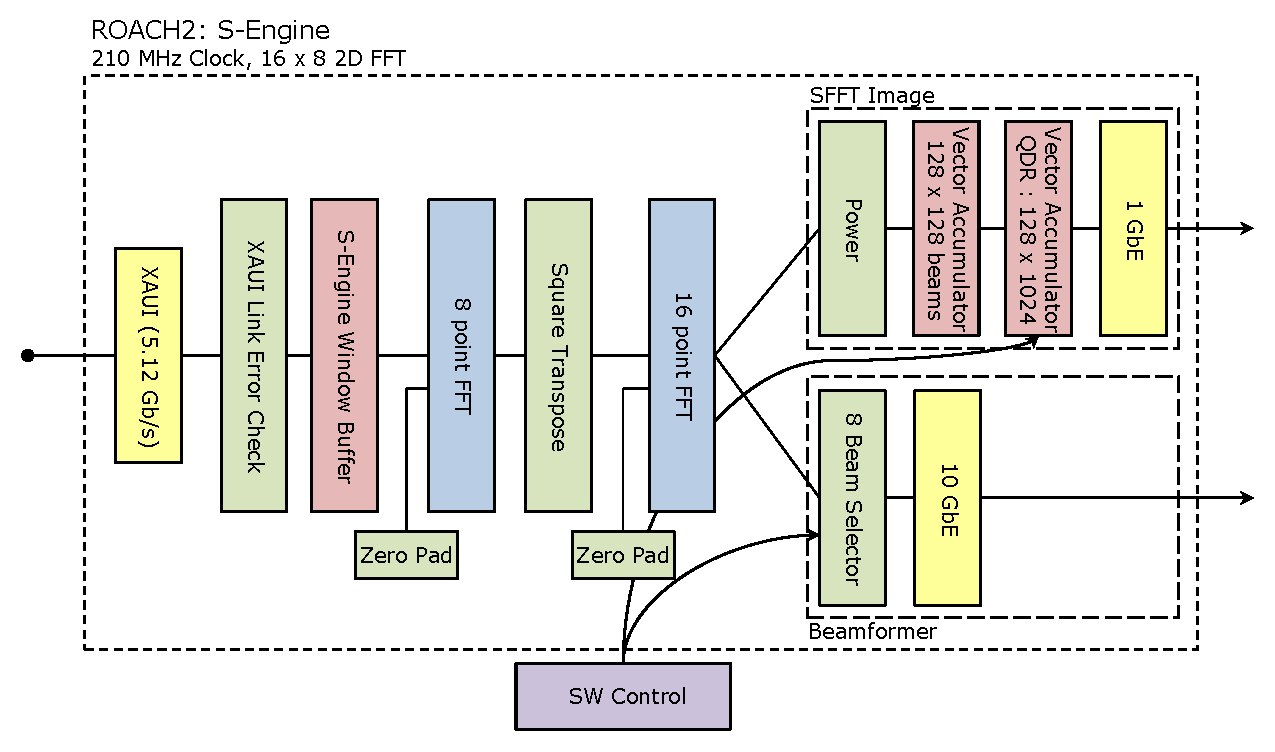
\includegraphics[scale=0.6]{graphics/crop_sengine_block.pdf}
    \caption{During the two stage spatial FFT the streams are zero padded to provide phase information of each baseline.}
    \label{fig:seng_block}
\end{figure}

\section{Deployment and Initial Observations}
\label{observations}

Instrumentation was installed and tested over a two week period in March 2012.
During that time a number of test signals were used to check the system status.
Once the system was checked out various bright radio sources were observed.
Since the Northern Cross is a transiting array there is a limited period of time each day in which a source is with the primary beam.
Bright sources such as Cygnus A, Cassiopeia A and Virgo A also with a number of 3C sources were observed along with multiple constant declination 24 hour cycles were observed.

Raw data from the correlator and imager was recorded to HDF5 files using a SPEAD protocol receive script.
A suite of python scripts have been written to interface and manipulate the data in this pre-calibration stage.
A python FITS-IDI package has been written to convert HDF5 files into the standard FITS format which can be read by AIPS and CASA\footnote{https://github.com/telegraphic/pyfitsidi}.
This allows for conversion to the Measurement Set format which most packages can interface with.

A number of calibration methods has been tested on the initial data sets.
Traditional CASA based calibration has been used to form correlator images.
To produce calibration coefficients for the spatial FFT imager a column ratio gain estimation method has been employed.
A study of the baseline redundancy and possible calibration has also been undertaken.
Long observations of the sky are under way to understand the system noise and our ability to reach the confusion limit.
During deep integration observations a cross talk issue covering part of the band has been discovered.

\subsection{Calibration Methods}
\label{calibration}

The effective averaging of redundant baselines in the spatial FFT imager requires complex gain calibrations to be applied during observations.
To derive gain coefficients a calibration method is applied to the FX correlator data.
In initial observations the column ratio gain estimation method from \citep{gaindecomp} was used to compute a per channel, per antenna complex gain term.

%SFFT correlations of Tau/3c144 before and after calibration
\begin{figure}
    \centering
    \subfloat[Dirty image of Tau/3c144 formed before applying complex gain calibrations in the F-Engine for the spatial FFT.]{
    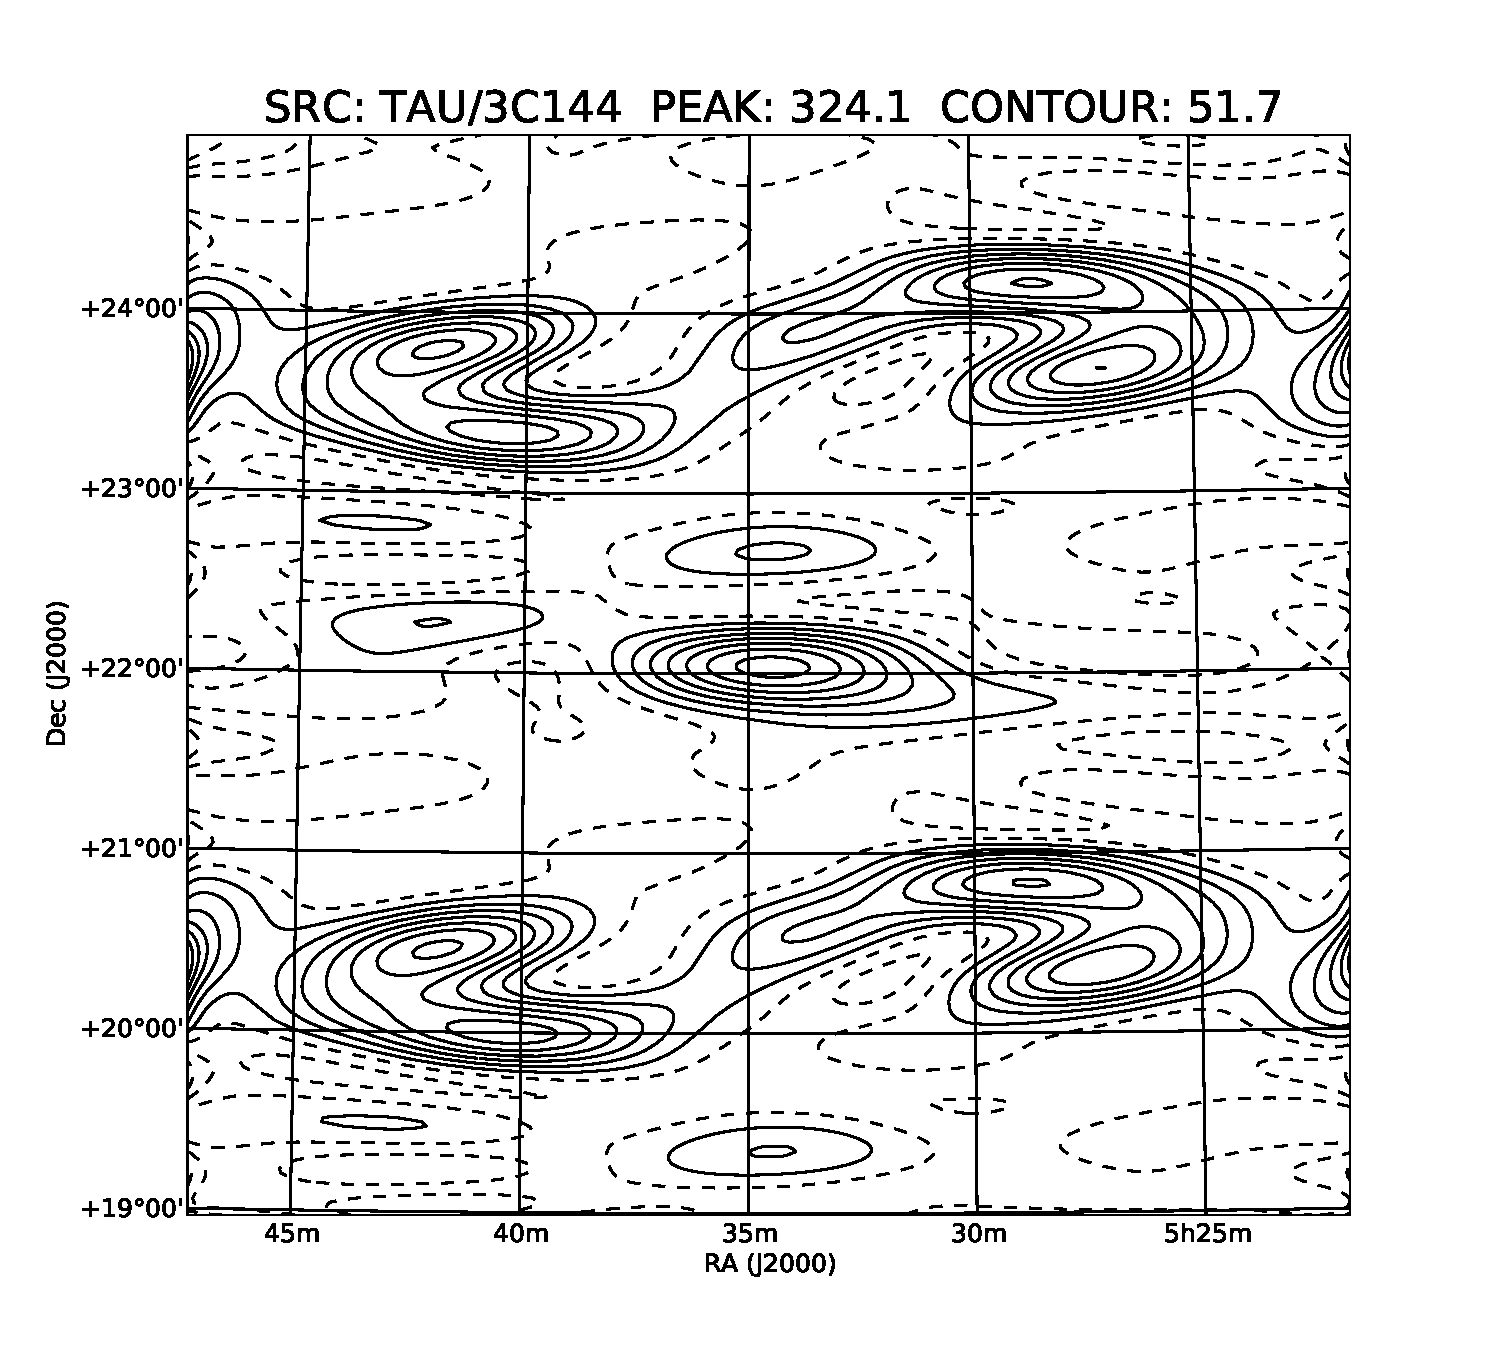
\includegraphics[scale=0.5]{{graphics/img.2455985.25525.tau.uncal.s.ms.DATA.channel.1ch}.pdf}
    \label{fig:uncal_sfft}
    }
    \hspace{10pt}
    \subfloat[Dirty image of Tau/3c144 with complex gain calibrations applied. This image has a signal to noise ratio around 20, a standard CLEAN method can be used to improve the image dynamic range.]{
    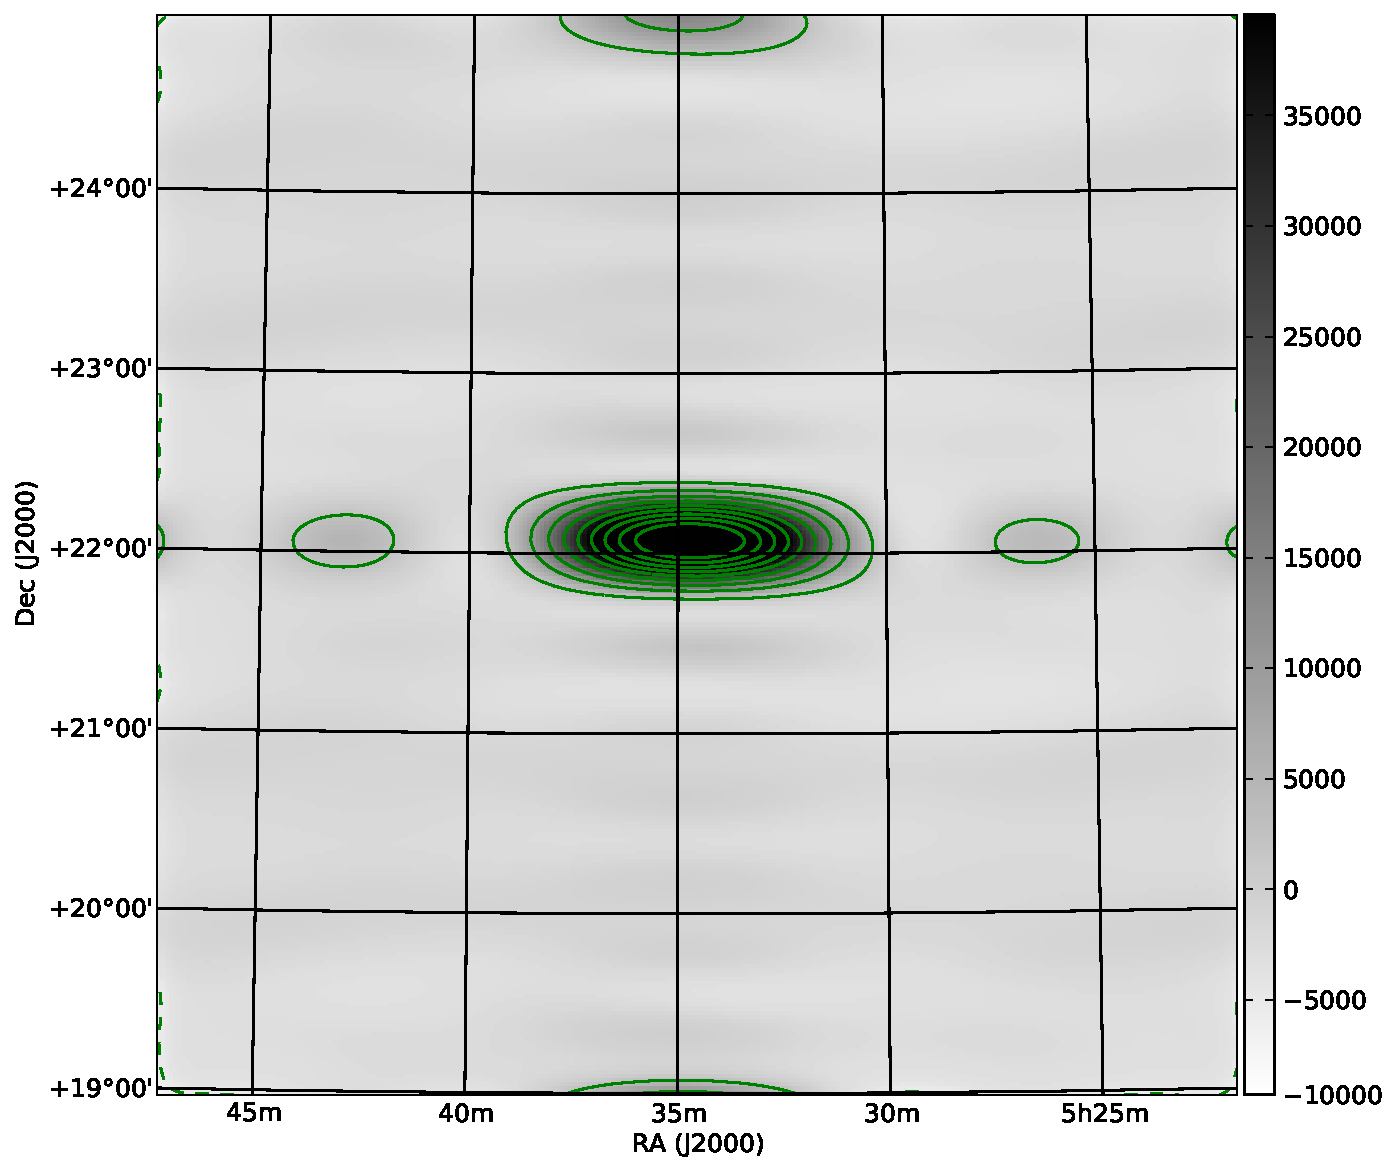
\includegraphics[scale=0.5]{{graphics/img.2455999.21403.tau.cal.s.ms.DATA.channel.1ch}.pdf}
    \label{fig:cal_sfft}
    }
    \label{fig:sfft_calibration}
    \caption{After applying complex gain calibration a bright point source such as Tau/3c144 appears similar to the array psf, and has a significant improvement in the image fidelity compared to the uncalibrated image.
    Scales in both images are based on raw spatial FFT visibilities.}
\end{figure}

\subsection{FX Correlator Imaging}
\label{fx results}

\begin{figure}
    \centering
    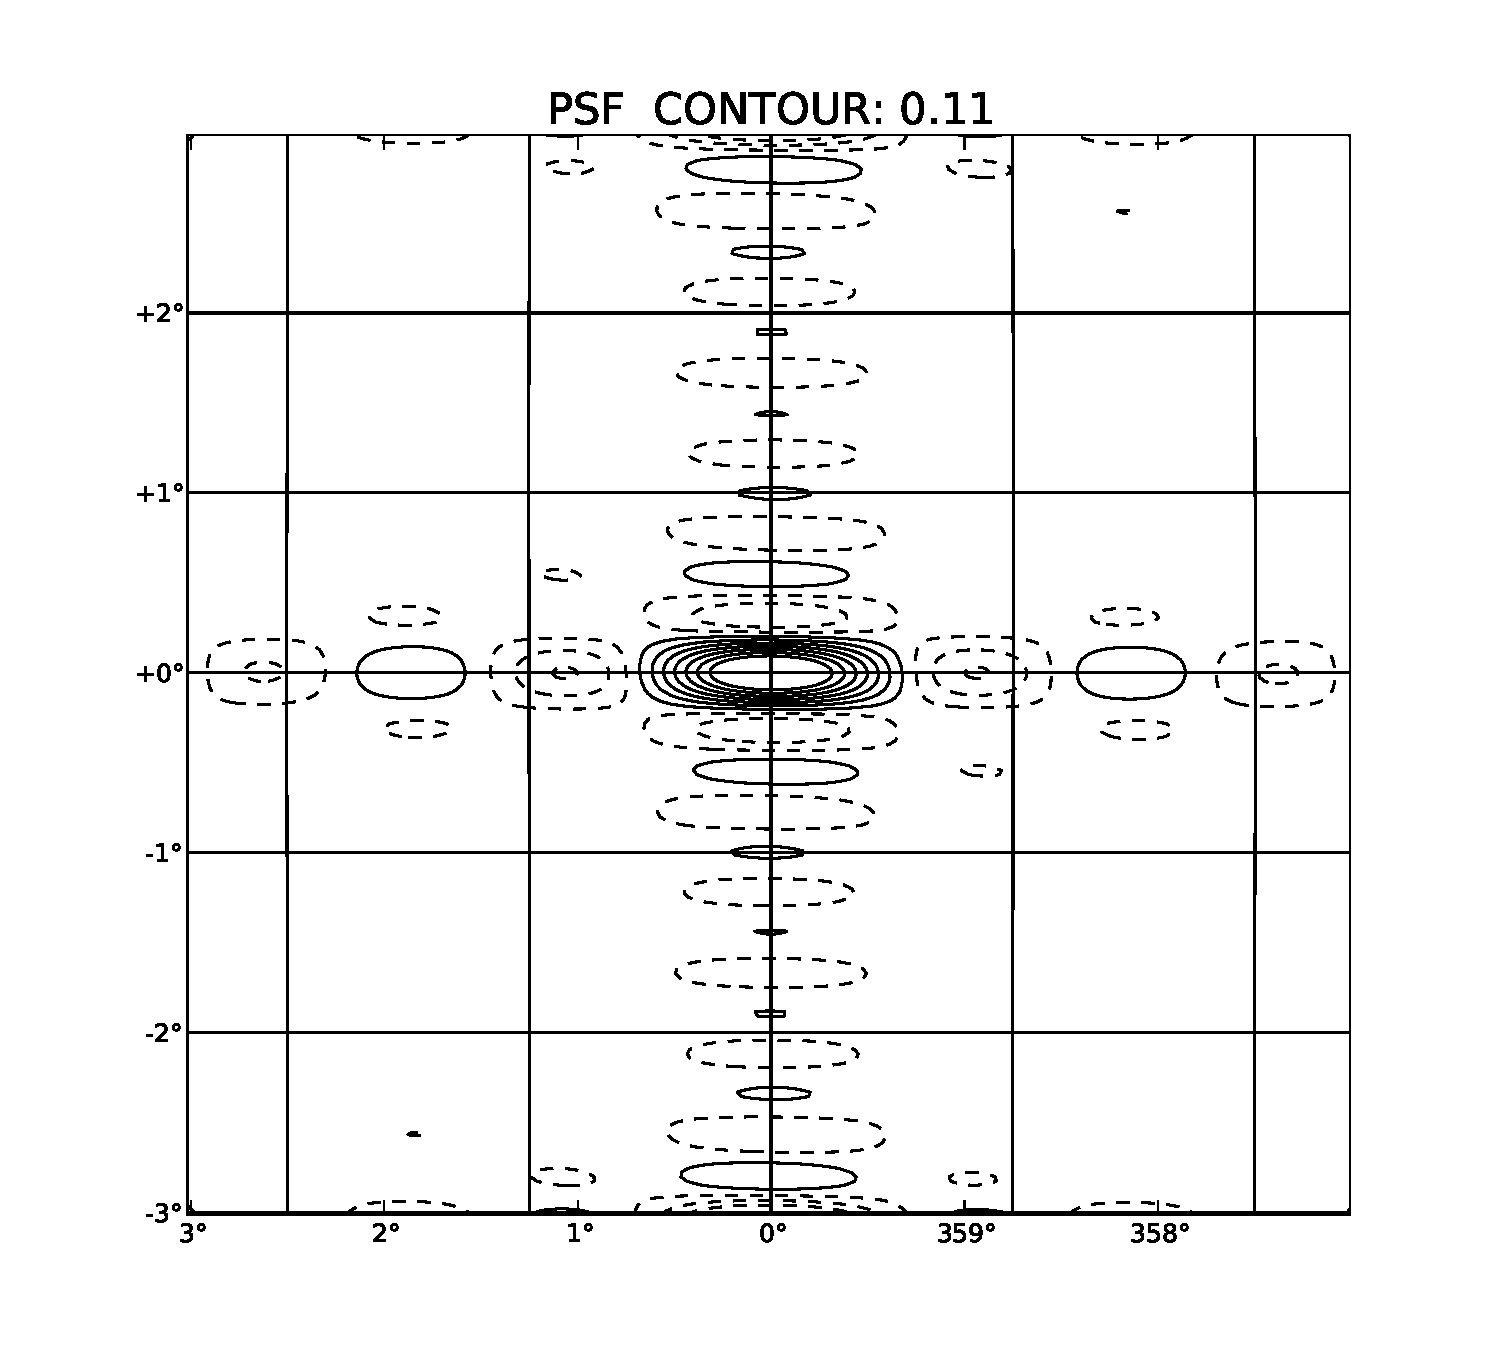
\includegraphics[scale=0.6]{{graphics/img.2455999.21403.tau.cal.s.ms.psf.channel.1ch.mod}.pdf}
    \caption{PSF of a two minute snapshot image.}
    \label{fig:psf}
\end{figure}

The East-West FWHM beam size of an individual element is $6.6^{\circ}$ which translates to a 26 minute 'transit time' for an source.
For the the bright A class sources this time can be extended since they remain the dominating source well after crossing the FWHM.
Observations of 40-50 minutes are possible which gives an improvement in uv coverage.
Initial calibration and imaging has been performed using the bright sources: Cygnus A, Cassiopeia A, Virgo A and Taurus A.

A transiting array provides a unique challenge of gain calibration since a source's apparent gain will change as it transits the primary beam.
A typical beam transit of a strong source, Cygnus A, is show in figure \ref{fig:gain_change}.
The auto correlations asymmetry is due to the changing galactic plane pass through the beam.
In the cross correlations the first and second sidelobes are evident.
Much of the sky surrounding a bright source is contaminated due to these high sidelobes.
The traditional method of using a gain calibrator is not possible.
Gain calibration of bright sources was done by fitting a solution on short time intervals.
A model of the beam will be necessary to set a better flux scale and time independent gain solution.

\begin{figure}
    \centering
    \subfloat[A selection of typical auto correlations over a period of five hours during a transit of Cygnus A. The asymmetry is due to the background galactic plane.]{
    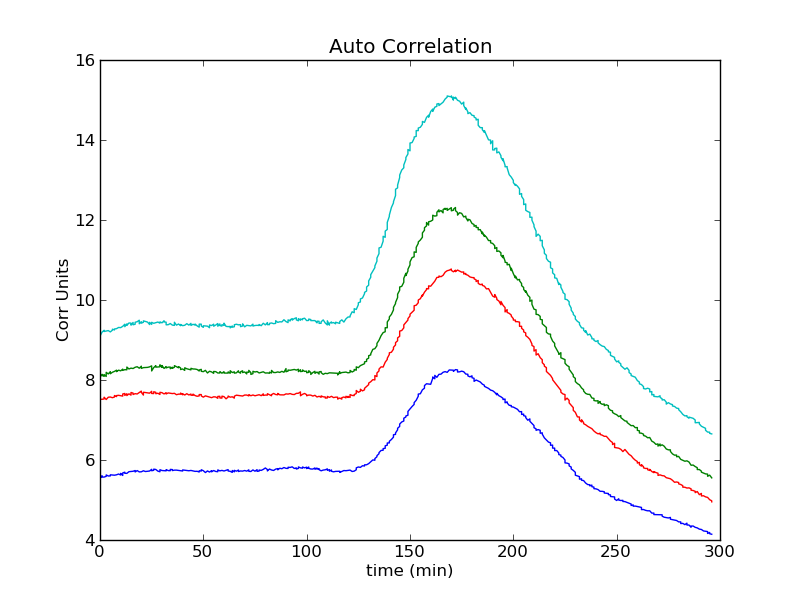
\includegraphics[scale=0.4]{graphics/gain_change_auto.png}
    \label{fig:gain_change_auto}
    }
    \hspace{10pt}
    \subfloat[Cross correlation power over a period of five hours during a Cygnus A transit. The first sidelobes are around 100 times lower then the primary lobe. A bright source like Cygnus A remains the dominant source in the field even into the second sidelobe.]{
    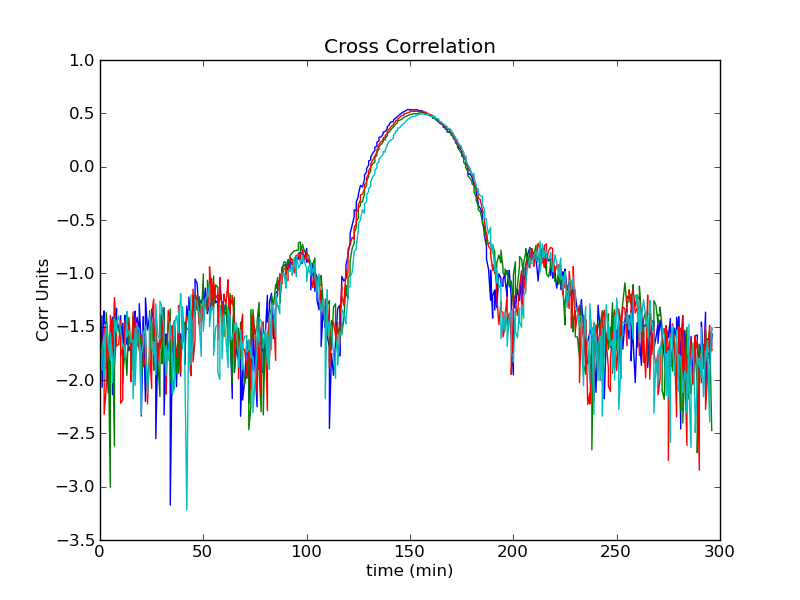
\includegraphics[scale=0.4]{graphics/gain_change_cross.png}
    \label{fig:gain_change_cross}
    }
    \label{fig:gain_change}
    \caption{Typical auto and cross correlations of a transiting source.}
\end{figure}

%Bright class A sources dominate the noise in a few seconds of integration.
%Images can be formed by taking short periods of time where the gain is effectively flat across the time interval.
%
%%casseopia a image from CASA
%\begin{figure}
%    \centering
%    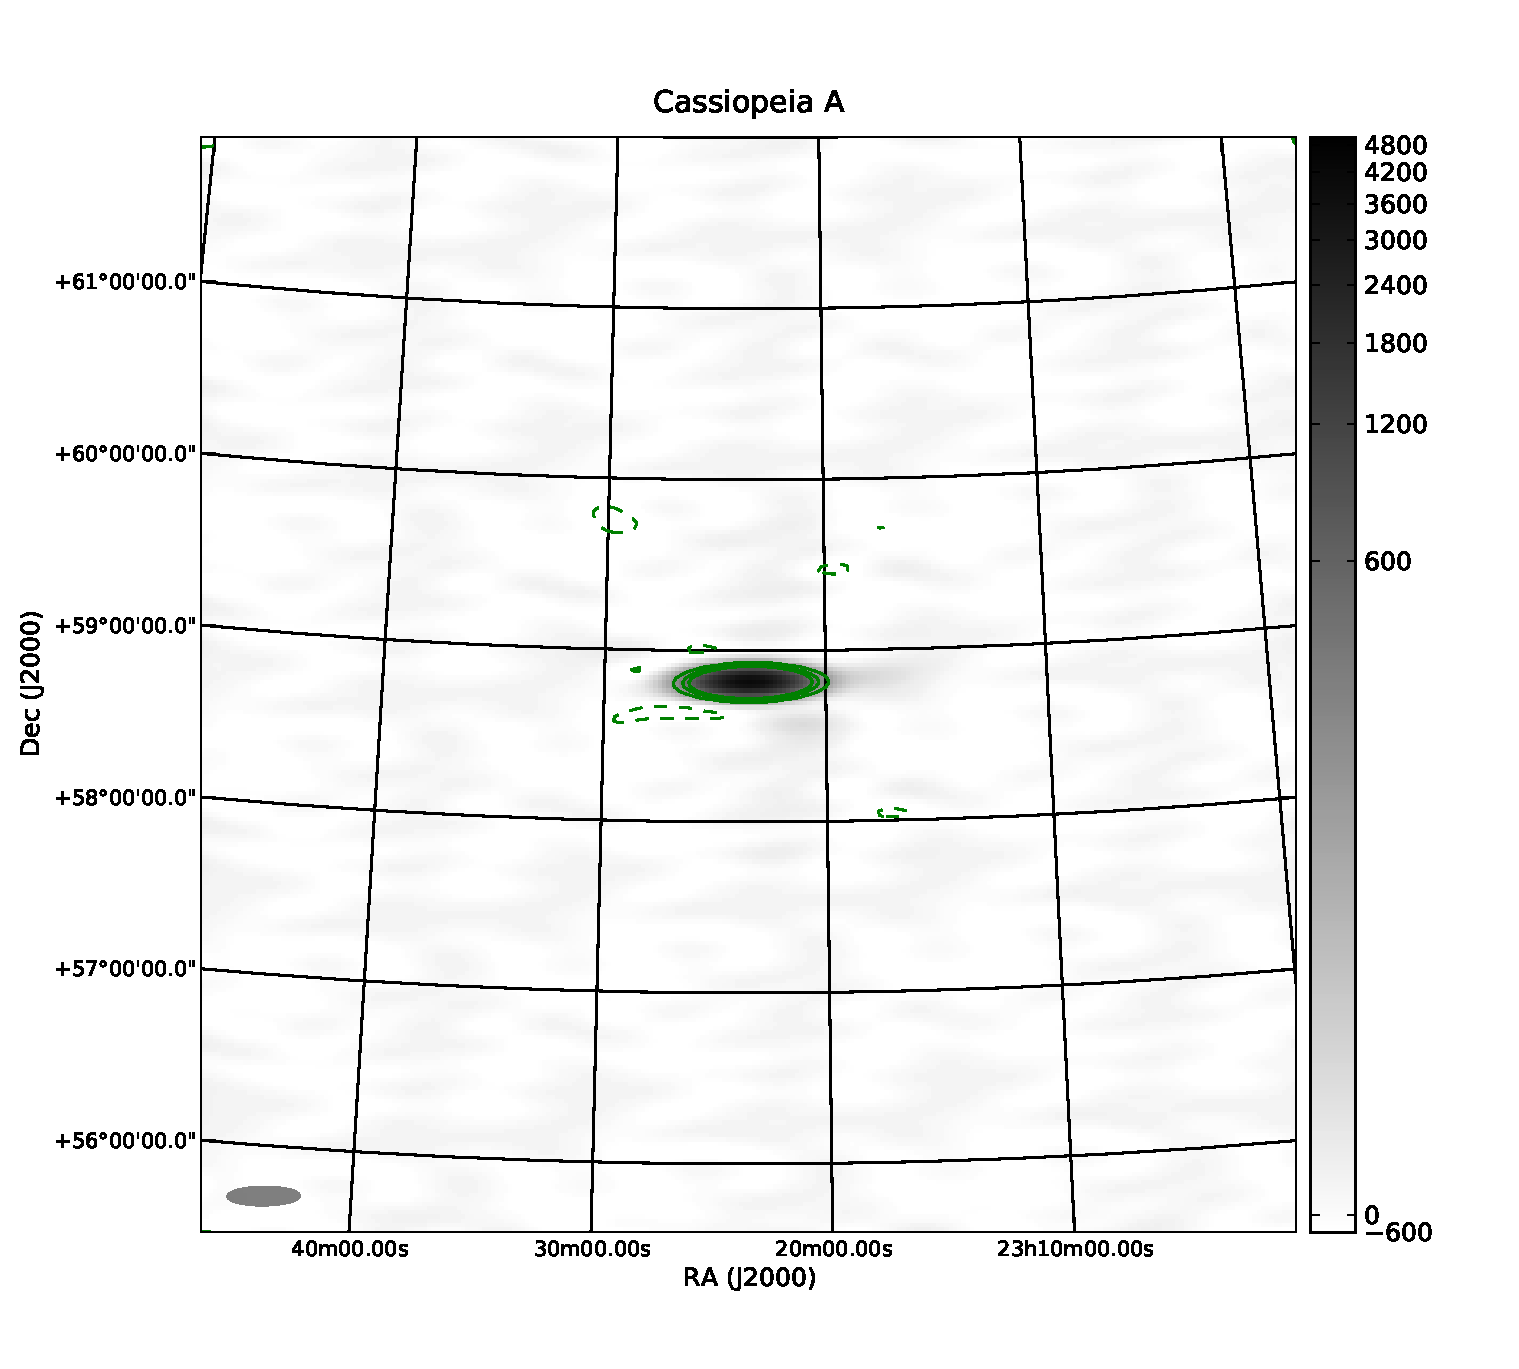
\includegraphics[scale=0.6]{graphics/cas_1319623663.pdf}
%    \caption{Calibrated image of Cassiopeia A using a 1 MHz portion of the band. This multi-frequency synthesis image was formed using a 40 minute transit of Cas A across the main lobe of the beam.
%    The two 'sources' above and below the main source are artifacts of the first sidelobe. Beam effects are currently a limiting factor in improving the dynamic range of the image.
%    The grayscale is Jy/Beam, with a nominal noise floor of $\approx 10$ Jy.}
%    \label{fig:cas_a_corr}
%\end{figure}
%
%Other sources, which are bright but a few orders of magnitude weaker than the class A sources have also been imaged.
%The bright 3C source 3C 196 can be imaged with 10's of seconds of integration.
%The flux scale on this source is off by a factor of approximately two because of our ability to set a flux scale based on a standard calibrator source and rely on a crude estimation using Cygnus A and Cassiopeia A.
%
%\begin{figure}
%    \centering
%    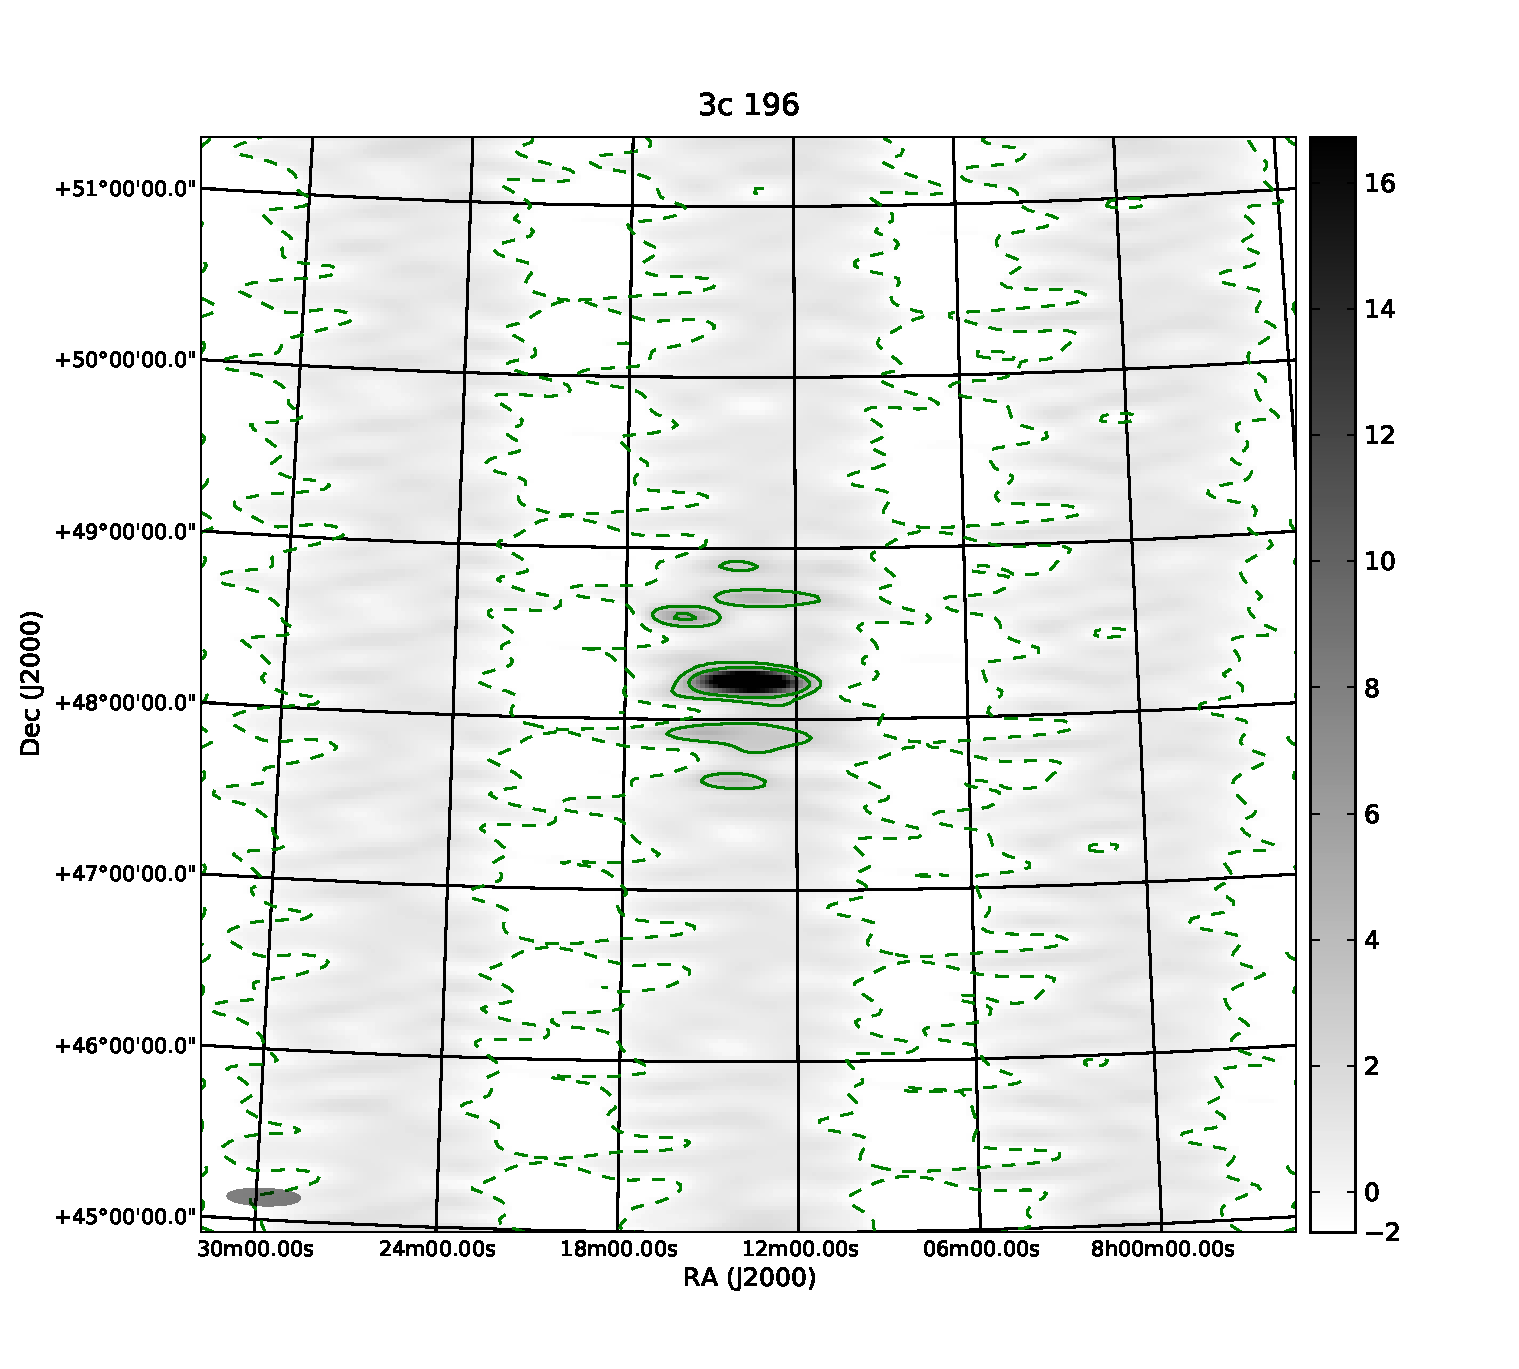
\includegraphics[scale=0.6]{graphics/3c196_01.pdf}
%    \caption{}
%    \label{fig:3c196_corr}
%\end{figure}

\subsection{Spatial FFT Results}
\label{sfft results}

%calibrated/uncalibrated images

\subsection{Comparison of FX Correlator and Spatial FFT}

%baselines
%images

%\subsection{Crosstalk Effects}
%\label{crosstalk}
%
%A strong cross talk effect has been observed in the lower portion of the band.
%This has the effect of creating a strong correlation, constant correlation across a few Megahertz before the effect tapers off below current noise measurements.
%Every baseline is affected to varying degrees, figure \ref{fig:xtalk}.
%The cross talk does not appear to be location or antenna dependent which suggests that it is not primarily from antenna coupling.
%A lab setup of the digital design has not been able to reproduce this effect but could still be related to the ADC cabling interface.
%Components with in the analogue chain could not be functioning within specification and causing the signal leakage.
%Further testing is required to discover the route of this issue.
%
%\begin{figure}
%    \centering
%    \subfloat[]{\label{fig:xtalka}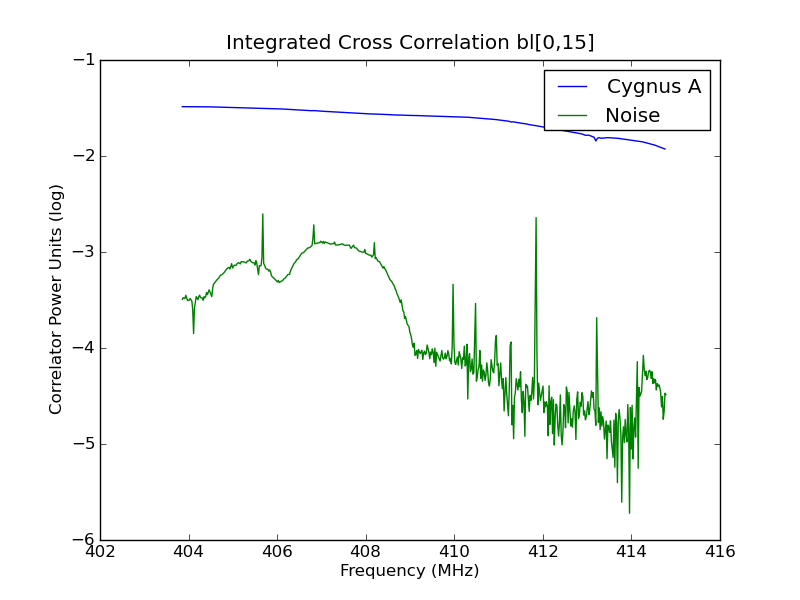
\includegraphics[width=0.3\textwidth]{graphics/xtalk/xtalk_plot_a.png}}
%    \subfloat[]{\label{fig:xtalkb}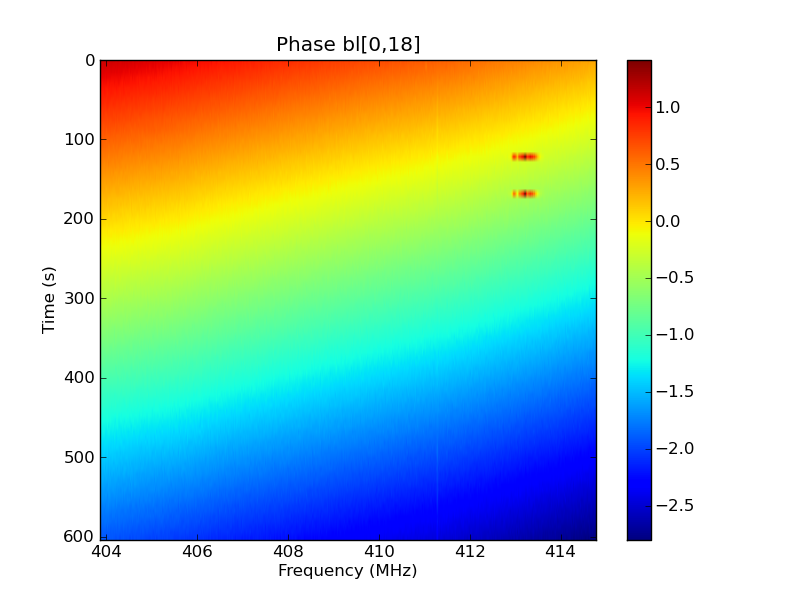
\includegraphics[width=0.3\textwidth]{graphics/xtalk/xtalk_plot_b.png}}
%
%    \subfloat[]{\label{fig:xtalkc}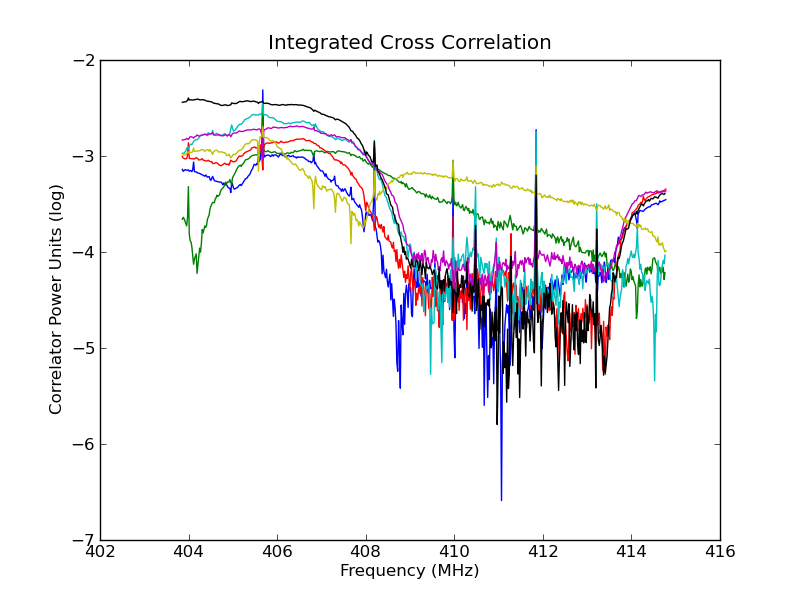
\includegraphics[width=0.3\textwidth]{graphics/xtalk/xtalk_plot_c.png}}
%    \subfloat[]{\label{fig:xtalkd}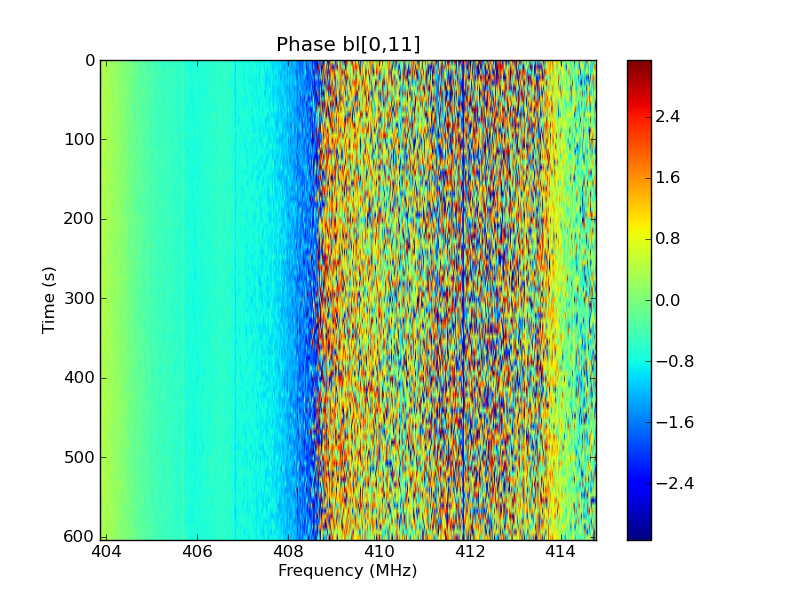
\includegraphics[width=0.3\textwidth]{graphics/xtalk/xtalk_plot_d.png}}
%    \caption{The lower portion of the band has a strong correlation effect caused by cross talk.
%    On observing strong sources the effect is weak but becomes a dominate effect when observing a cold patch of the sky, fig. \ref{fig:xtalka}.
%    Cross talk is noticeable in almost all the cross correlations, fig. \ref{fig:xtalkc} shows a handful of baselines.
%    This effect is difficult to localize, there is no obvious systematic effects with regard to antenna locations or cabling.
%    Figure \ref{fig:xtalkb} is a phase plot (Radians) of the observation of bright source.
%    Figure \ref{fig:xtalkd} is a phase plot of a region with no sources, the cross talk has the effect of flattening the lower end of the band.}
%    \label{fig:xtalk}
%\end{figure}

\section{Discussion}
\label{discussion}

%what has been accomplished
%further work on BEST-2: noise floor
%further work: spatial FFT

\bibliography{refs}{}
\bibliographystyle{mn2e}

%\newpage
%\begin{thebibliography}{9}
%
%\bibitem[\protect\citeauthoryear{Boonstra}{2001}]{gaindecomp}
%A.J. Boonstra and A.J. Van der Veen,
%"Gain Decomposition Methods for Radio Telescope Arrays", 2001
%\emph{IEEE Workshop on Statistical Signal Processing (SSP)}, Singapore, August 2001
%
%\bibitem[\protect\citeauthoryear{Montebugnoli}{2009}]{best2}
%S. Montebugnoli, G. Bianchi, J. Monari, G. Naldi, F. Perini, and M. Schiaffino,
%"BEST: Basic Element for SKA Training", 2009
%\emph{SKADS Conference 2009: Widefield Science and Technology for the SKA}, p. 331-336
%
%\bibitem[\protect\citeauthoryear{Montebugnoli}{2009}]{best2-casper}
%S. Montebugnoli, M. Bartolini, G. Bianchi, G. Naldi, J. Manley, and A. Parsons,
%"BEST Back End", 2009
%\emph{SKADS Conference 2009: Widefield Science and Technology for the SKA}, p. 355-358
%
%\bibitem[\protect\citeauthoryear{Otobe}{1994}]{2dfft}
%E. Otobe, J. Nakajima, K. Nishibori, T. Saito, H. Kobayashi, N. Tanaka, N. Watanabe, Y. Aramaki, T. Hoshikawa, K. Asuma, and T. Daishido,
%"Two-dimensional Direct Images with a Spatial FFT Interferometer", 1994,
%\emph{PASJ}, Vol. 46, No. 5, p. 503-510
%
%\bibitem[\protect\citeauthoryear{Perini}{2009}]{best2-rec}
%F. Perini, G. Bianchi, M. Schiaffino, and J. Monari,
%"BEST Receiver Experience: General Architecture, Design and Integration", 2009
%\emph{SKADS Conference 2009: Widefield Science and Technology for the SKA}, p. 351-354
%
%\bibitem[\protect\citeauthoryear{Perini}{2009}]{best2-lna}
%F. Perini,
%"Low Noise Design Experience for the SKADS/BEST Demonstrator", 2009
%\emph{SKADS Conference 2009: Widefield Science and Technology for the SKA}, p. 341-345
%
%\bibitem[\protect\citeauthoryear{Parsons et al.}{2009}]{casper}
%A. Parsons, D. Backer, C. Chang, D. Chapman, H. Chen, P. Crescini, C. de Jesus, C. Dick, P. Droz, D. MacMahon, K. Meder, J. Mock,
%V. Nagpal, B. Nikolic, A. Parsa, B. Richards, A Siemion, J. Wawrzynek, D. Werthimer, M. Wright,
%"PetaOp/Second FPGA Signal Processing for SETI and Radio Astronomy", 2006
%\emph{Asilomar Conference on Signals and Systems, Pacific Grove, CA}, p. 2031-2035
%
%\end{thebibliography}

\end{document}
